% latex-ops example: Minimal Beamer.
% Prompt: "Turn the gradient-descent note into a 5-minute talk, 16:9."
\documentclass[aspectratio=169,14pt]{beamer}

\usepackage[english]{babel}
\usepackage{fontspec}
\usepackage{unicode-math}
\usepackage{microtype}
\usepackage{booktabs}
\usepackage{pgfplots}
\pgfplotsset{compat=1.18}

\IfFontExistsTF{Inter}{\setsansfont{Inter}}{\setsansfont{Latin Modern Sans}}
\usefonttheme{professionalfonts}
\setmathfont{Latin Modern Math}

% Semantic colours: emphasis only, AA contrast on white; meaning never rests on colour alone.
\definecolor{Ink}{HTML}{1F2A30}
\definecolor{Accent}{HTML}{315B6B}
\definecolor{Muted}{HTML}{6B6B6B}
\newcommand{\HL}[1]{{\color{Accent}\bfseries #1}}
\newcommand{\HLmath}[1]{\textcolor{Accent}{#1}}

\setbeamercolor{normal text}{fg=Ink}
\setbeamercolor{frametitle}{fg=Ink}
\setbeamercolor{title}{fg=Ink}
\setbeamercolor{subtitle}{fg=Muted}
\setbeamercolor{footline}{fg=Muted}
\setbeamerfont{title}{size=\huge,series=\bfseries}
\setbeamerfont{frametitle}{size=\Large,series=\bfseries}
\setbeamertemplate{navigation symbols}{}
\setbeamertemplate{footline}{\hfill\usebeamerfont{footline}\usebeamercolor[fg]{footline}\insertframenumber\hspace{1.2em}\vspace{.8em}}
\setbeamertemplate{itemize item}{\color{Accent}--}
\setbeamersize{text margin left=2.2em,text margin right=2.2em}

\title{How fast does gradient descent converge?}
\subtitle{Strongly convex quadratics in five minutes}
\author{A.\ Example}
\date{}

\begin{document}

\begin{frame}[plain]
  \vfill\titlepage\vfill
  {\footnotesize\color{Muted}Illustrative example generated with latex-ops.\par}
\end{frame}

\begin{frame}{Why it matters}
  \begin{itemize}\setlength{\itemsep}{.8em}
    \item Training a model means running an optimiser for many steps.
    \item The question is not \emph{whether} it converges but \HL{how many steps} it needs.
    \item For quadratics the answer is exact and depends on one number.
  \end{itemize}
\end{frame}

\begin{frame}{The condition number decides}
  \[
    f(x) = \tfrac12 x^\top A x - b^\top x, \qquad \mu I \preceq A \preceq L I, \qquad
    \kappa = \frac{L}{\mu}
  \]
  \vspace{.6em}
  With step $\eta = 2/(L+\mu)$:
  \[
    \lVert x_k - x^\star \rVert \le \HLmath{\left(\frac{\kappa-1}{\kappa+1}\right)^{k}}
    \lVert x_0 - x^\star \rVert
  \]
\end{frame}

\begin{frame}{10× worse conditioning, 10× more steps}
  \begin{columns}[T]
    \begin{column}{.6\textwidth}
      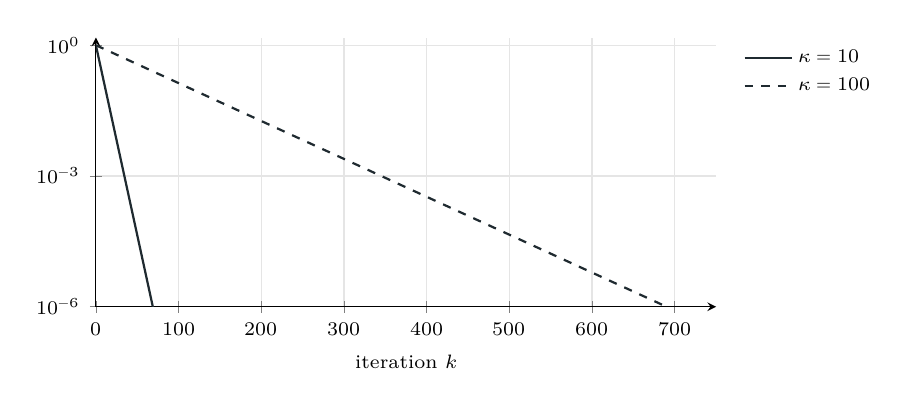
\begin{tikzpicture}
      \begin{semilogyaxis}[
        width=.78\linewidth, height=5cm, xmin=0, xmax=750, ymin=1e-6, ymax=1.5,
        xlabel={iteration $k$}, axis lines=left, grid=major, grid style={gray!20},
        tick label style={font=\scriptsize}, label style={font=\scriptsize},
        legend style={font=\scriptsize, draw=none}, legend pos=outer north east,
        legend cell align=left]
        \addplot[Ink, thick, domain=0:750, samples=300] {(9/11)^x};
        \addlegendentry{$\kappa=10$}
        \addplot[Ink, thick, dashed, domain=0:750, samples=300] {(99/101)^x};
        \addlegendentry{$\kappa=100$}
      \end{semilogyaxis}
      \end{tikzpicture}
    \end{column}
    \begin{column}{.36\textwidth}
      \vspace{1em}\small
      \begin{tabular}{rr}
        \toprule
        $\kappa$ & steps to $10^{-6}$ \\
        \midrule
        10 & 69 \\
        100 & 691 \\
        1000 & 6908 \\
        \bottomrule
      \end{tabular}
    \end{column}
  \end{columns}
\end{frame}

\begin{frame}{Takeaways}
  \begin{itemize}\setlength{\itemsep}{.8em}
    \item Gradient descent on quadratics converges \HL{linearly}.
    \item Steps grow roughly like $\tfrac{\kappa}{2}\ln(1/\varepsilon)$.
    \item Better conditioning (preconditioning, rescaling) pays off directly.
  \end{itemize}
\end{frame}

\end{document}
